\documentclass{article}
\usepackage[latin1]{inputenc}
\usepackage[norsk]{babel}
\usepackage{amsmath}
\usepackage{mathabx}
\usepackage{graphicx}
\usepackage{caption}
\usepackage{subcaption}
\usepackage{float}
\usepackage{color}
%\usepackage{geometry}
% \geometry{
% a4paper,
% total={170mm,257mm},
% left=10mm,
% top=10mm,
% }
\title{Project 3 - Fys3150}
\author{Anders Huse Pedersen}
\begin{document}
\section*{abstract}
The orbit of a planet is an ellipse with the Sun at one of the two foci. Using the method from Euler and Verlet, we can perform a decent simulation of this system, but the algorithm's have their advantages and disadvantages. It turns out ... so the conclusion is ...
\section{Solar system}
The solar system is the gravitationally bound system compromising the Sun and the objects that orbit it either directly or indirectly. Planets and smaller solar system bodies are said to directly orbitting the Sun while moons are said to indirectly orbitting the Sun.
According to kepler's law, each object travels along an ellipse with the Sun at on focus. On an elliptic orbit, a body's distance from the Sun varies over the course of its year. A body's closest approach to the Sun is called perihelion, while the it's most distant point from the Sun is called its aphelion.
\subsection{Celestial mechanics}
Celestial mechanics is the branch of astronomy that deals with the motions of celestial objects. The basic equations which govern the solar system is are rather simple, a set of coupled equations that codify Newton's law of motion due to the gravitational force. In the first part of this project we'll concider a simplyfied two-body system where the Earth is the only planet orbiting the Sun. Gravity is the only force in this problem and Newton's law of gravitation is given by a force:
\begin{align*}
  F_G &= \frac{GM_{\Sun}m_{\Earth}}{r^2}\\
\end{align*}
where G is the gravitational force, r is the distance between the Earth and the Sun, $M_{\Sun}$ is the mass of the Sun and $m_{\Earth}$ is the mass of the Earth. Since $M_{\Sun} \gg m_{\Earth}$, we're neglecting the motion of the Sun. We also assume that the motion of the Earth around the Sun is co-planar using the xy-plane.
According to Newton's second law of motion (using x,y as the component of the force):
\begin{align*}
  \frac{d^2x}{dt^2} &= \frac{F_{G,x}}{m_{\Earth}}\\
  \frac{d^2y}{dt^2} &= \frac{F_{G,y}}{m_{\Earth}}\\
\end{align*}
For practical reasons we're measuring distance in AU (Astronomical Unit), masses in $M_{\Sun}$ and time in years.
Since the orbit of the Earth around the Sun is almost circular we also have the relation:
\begin{align*}
  F_{G} &= \frac{M_{\Earth}v^2}{r} = \frac{GM_{\Sun}m_{\Earth}}{r^2}\\
\end{align*}
where v is the velocity of the Earth.
Using simple algebra on this equation will give an expression for G, which is useful:
\begin{align*}
  v^2 r &= GM_{\Sun} = 4\pi^2 AU^3/yr^2\\
\end{align*}
To get the x and y components of the force we can multiply with $r \cos\theta/r\to x_{rel}/r$ and $r \sin\theta/r\to y_{rel}/r$:
\begin{align*}
  F_{G,x} &=F_{G}\cdot \frac{r \cos\theta}{r}= \frac{GM_{\Sun}m_{\Earth} x_{rel}}{r^3}\\
  F_{G,y} &=F_{G}\cdot \frac{r \sin\theta}{r}= \frac{GM_{\Sun}m_{\Earth} y_{rel}}{r^3}\\
\end{align*}
where $\theta$ is the angular position of the Earth in the solar referencal.
Substituting back into our differential equations gives:
\begin{align*}
  \frac{d^2x}{dt^2} &= \frac{F_{G,x}}{m_{\Earth}}\\
  &= \frac{GM_{\Sun}x_{rel}}{r^3}\\
  \frac{d^2y}{dt^2} &= \frac{F_{G,y}}{m_{\Earth}}\\
  &= \frac{GM_{\Sun}y_{rel}}{r^3}\\
\end{align*}
Then we define the position $x(t)$ and velocity as its derivative $dx/dt=v(t)$, so that we can
rewrite our second order differential equation into two coupled first order differential equations:
\begin{align*}
  \frac{dx(t)}{dt} &= v(t)\\
  \frac{dv(t)}{dt} &= \frac{GM_{\Sun}x_{rel}}{r^3}\\
\end{align*}
Using the same approach for $y(t)$ we obtain:
\begin{align*}
  \frac{dy(t)}{dt} &= v(t)\\
  \frac{dv(t)}{dt} &= \frac{GM_{\Sun}y_{rel}}{r^3}\\
\end{align*}
\subsection*{Euler's Forward}
We want to discretize this equation in order to be able to solve it numerically, so we define the following step size:
\begin{align*}
  h &= \frac{b-a}{N}
\end{align*}
where $a$ is the start time, $b$ is the final time and N is the number of integration points.
To write our algorithm we write our second order differential equations in terms of two first order equation to obtain:
\begin{align*}
  \frac{d^2x}{dt^2} &= \frac{F_{G,x}}{m_{\Earth}}\\
  &= \frac{GM_{\Sun}x_{rel}}{r^3}\\
\end{align*}
To discretize our equations, we define the step size to be:
\begin{align*}
  h &= \frac{b-a}{N}\\
\end{align*}
We are also given an initial value $x_0 = 1AU$ for the function $x(t)$ so we can write $x_0 = x(t = t_0)$.
Using the derivative of x and the time step we can find the next value:
\begin{align*}
  x_1 &= x(t_1) = x(t_0+h)\\
\end{align*}
We can continue in this way to find the next step:
\begin{align*}
  x_{n+1} &= x(t=t_i+h)\\
  &=x(t_i)+h\Delta(t_i,x_i(t_i))+\underbrace{O(h^{p+1})}_{\text{Truncation error}}\\
\end{align*}
Using Taylor expansion on our function (truncated at first derivative) gives $\Delta= x'(t_i)$ and a truncation error $O(h^{p+1} = O(h^2)$ at every step. The total error is $(b-a)/h\cdot O(h2) \approx O(h)$.
Finally, we have the algorithm for Euler's Forward method:
\begin{align*}
  x_{n+1} &= x_n + hv_n\\
  v_{n+1} &= v_n + ha_n\\
\end{align*}
{\color[rgb]{1,0,0}SKRIV ALGORITME}
\subsection*{Velocity Verlet}
We use Taylor expansion again for $x(t\pm h)$ and truncate at the second derivative. Then we add the two equations together:
\begin{align*}
  x(t+h) &= x(t)+hx'(t)+\frac{h^2}{2}x''(t)+O(h^3)\\
  x(t-h) &= x(t)-hx'(t)+\frac{h^2}{2}x''(t)+O(h^3)\\
  x(t+h)+x(t-h) &= x(t)+x(t)+hx'(t)-hx'(t)+\frac{h^2}{2}x''(t)+\frac{h^2}{2}x''(t))+O(h^4)\\
  x(t+h) &= 2x(t)-x(t-h)+h^2x''(t)+O(h^4)\\
\end{align*}
The odd terms cancel, so that the error is $O(h^4)$.
Discretizing this using $x(t_i\pm h = x_{i\pm 1}$ and $x_i = x(t_i)$ give us the Verlet method: 
\begin{align*}
  x_{n+1} &= 2x_n-x_{n-1}+h^2a_n+O(h^4)\\
  y_{n+1} &= 2y_n-y_{n-1}+h^2a_n+O(h^4)\\
\end{align*}
where we have used that $x''(t) = a(x,t)$.
SKRIV ALGORITME
\newpage
\section*{c) Test of Algorithm}
We have placed the Sun (red dot) at $(x,y) = (0,0)$ 
When $v_y(t_0) = 2\pi$ the orbits are about circular. 
\begin{figure}[H]
  \centering
  \begin{subfigure}{0.5\textwidth}
    \centering
    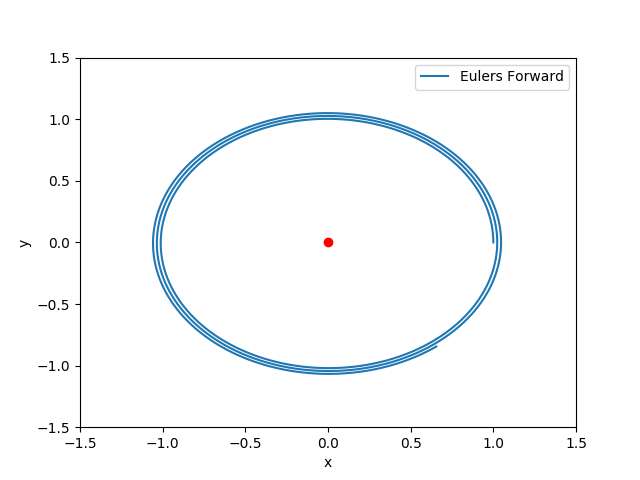
\includegraphics[width=1.0\textwidth]{plots/euler_v_2pi_h10000_t3.png}
    \caption{Euler's Forward \\(N: 10000, time: 3yr)}
  \end{subfigure}%
  \begin{subfigure}{0.5\textwidth}
    \centering
    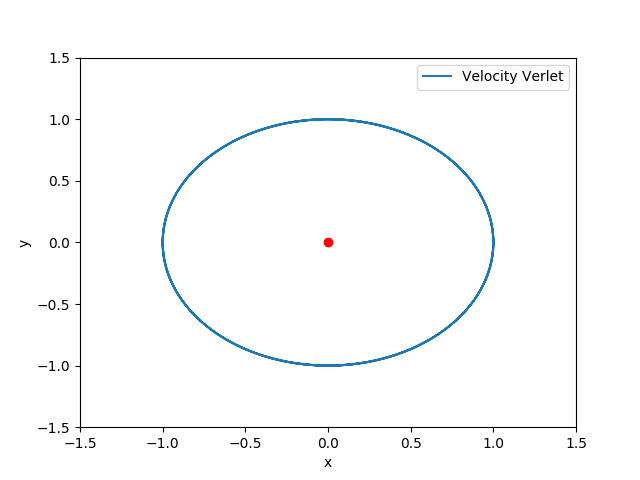
\includegraphics[width=1.0\textwidth]{plots/verlet_v_2pi_h10000_t3.png}
    \caption{Velocity Verlet \\(N: 10000, time: 3yr)}
  \end{subfigure}
\end{figure}

\subsection*{Testing different time steps}
\begin{figure}[H]
  \centering
      \begin{subfigure}{0.5\textwidth}
    \centering
    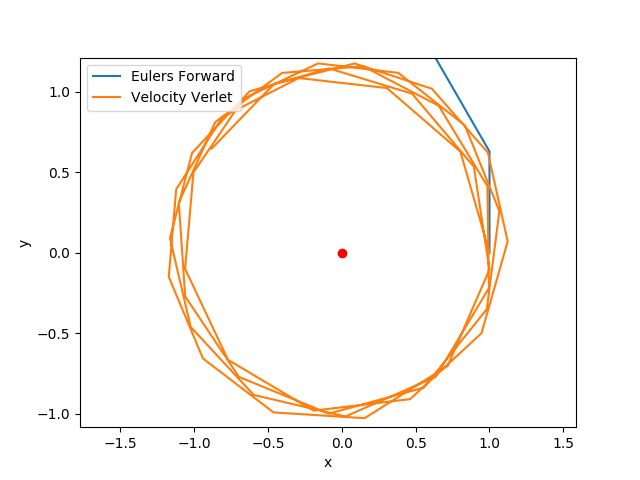
\includegraphics[width=1.0\textwidth]{plots/compare_h1.png}
    \caption{step size: 0.1, time: 5yr, N:50}
  \end{subfigure}%
  \begin{subfigure}{0.5\textwidth}
    \centering
    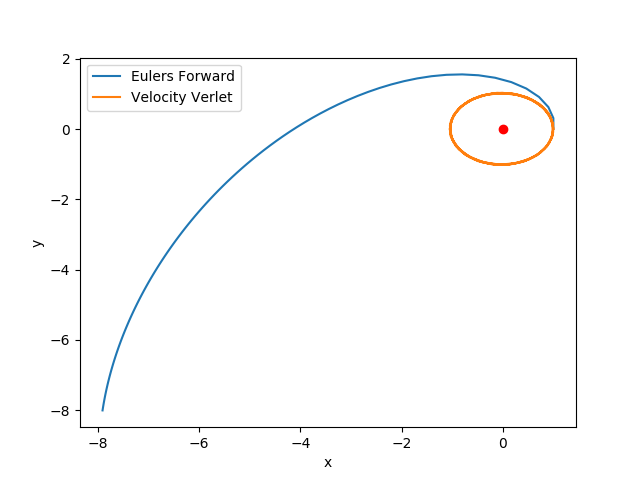
\includegraphics[width=1.0\textwidth]{plots/compare_h05.png}
    \caption{step size: 0.05, time: 5yr, N:100}
  \end{subfigure}
\end{figure}
\begin{figure}[H]
  \centering
  \begin{subfigure}{0.5\textwidth}
    \centering
    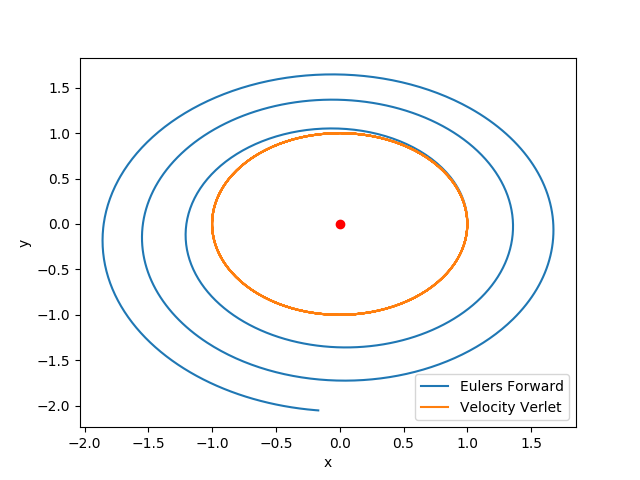
\includegraphics[width=1.0\textwidth]{plots/compare_h005.png}
    %\caption{Euler's Forward \\(stepsize: 10000, time: 3yr)}
  \end{subfigure}%
  \begin{subfigure}{0.5\textwidth}
    \centering
    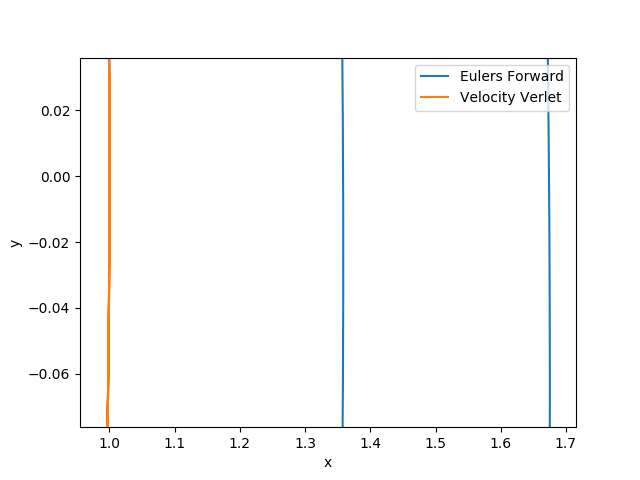
\includegraphics[width=1.0\textwidth]{plots/compare_h005_zoom.png}
    %\caption{Velocity Verlet \\(stepsize: 10000, time: 3yr)}
  \end{subfigure}
  \caption{step size: 0.005,time: 5yr, N: 1000}
\end{figure}
\begin{figure}[H]
  \centering
  \begin{subfigure}{0.5\textwidth}
    \centering
    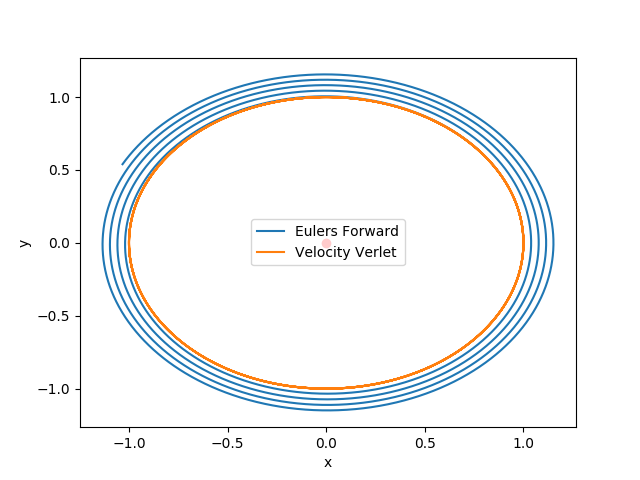
\includegraphics[width=1.0\textwidth]{plots/compare_h0005.png}
    %\caption{Euler's Forward \\(stepsize: 10000, time: 3yr)}
  \end{subfigure}%
  \begin{subfigure}{0.5\textwidth}
    \centering
    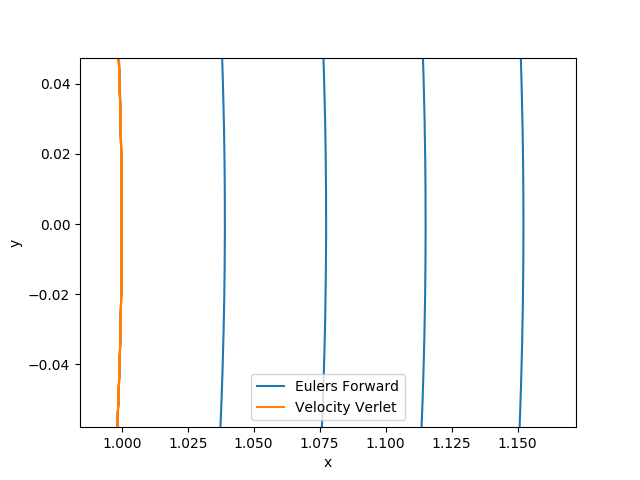
\includegraphics[width=1.0\textwidth]{plots/compare_h0005_zoom.png}
    %\caption{Velocity Verlet \\(stepsize: 10000, time: 3yr)}
  \end{subfigure}
  \caption{step size: 0.0005, time: 5yr, N: 10000}
\end{figure}
\begin{figure}[H]
  \centering
  \begin{subfigure}{0.5\textwidth}
    \centering
    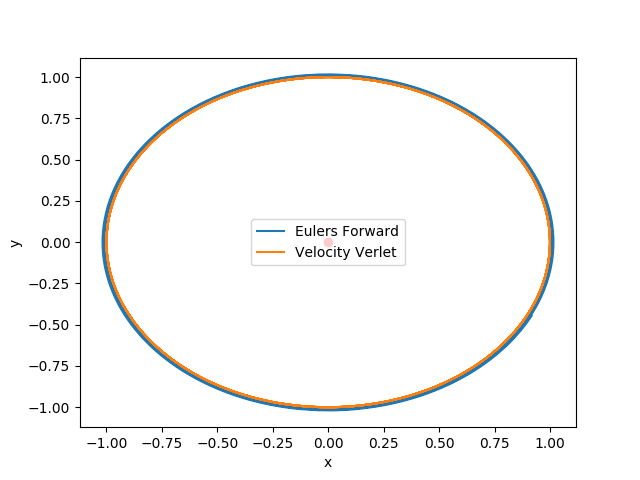
\includegraphics[width=1.0\textwidth]{plots/compare_h00005.png}
    %\caption{Euler's Forward \\(stepsize: 10000, time: 3yr)}
  \end{subfigure}%
  \begin{subfigure}{0.5\textwidth}
    \centering
    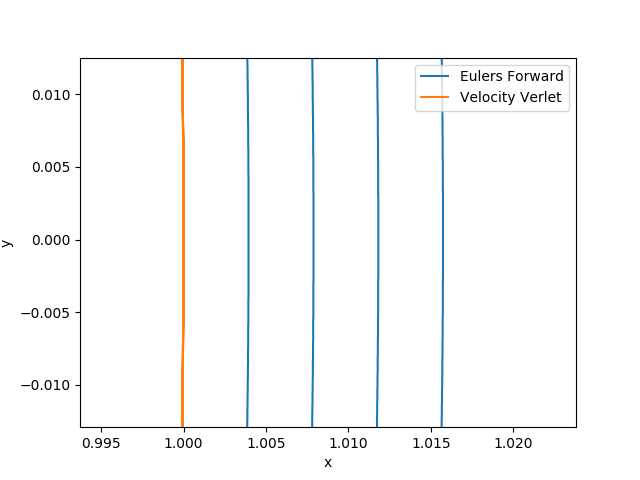
\includegraphics[width=1.0\textwidth]{plots/compare_h00005_zoom.png}
    %\caption{Velocity Verlet \\(stepsize: 10000, time: 3yr)}
  \end{subfigure}
  \caption{step size: 0.00005, time: 5yr, N: 100000}
\end{figure}
As we can see the Euler's Forward method gives a poor result even for low stepsize, while Velocity Verlet is very impressive. Even at step size of 0.1 you'll get the tendency of a circular and stable orbit even though it gets displaced. But decreasing the step size to 0.05 or 0.005 seems to be enough to get a reasonable result. In the Euler method the energy is not conserved. It is increasing. In this method $v(i)$ is expressed in terms of the previous steps. For time steps that are too large, this causes the computed solution to deviate significantly from the true solution. If the differential equation is too stiff, avoiding this problem might require time steps so small that it would not be computaionally viable.
\subsection*{Energy of the Sun-Earth system}
\begin{figure}[H]
  \centering
  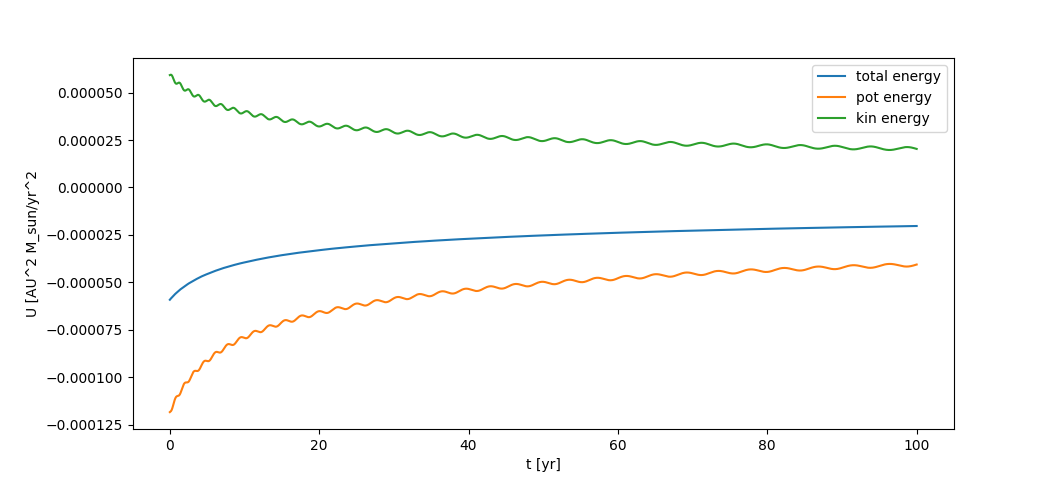
\includegraphics[width=1.0\textwidth]{plots/euler_energysystem100yr.png}
  \caption{Euler's Forward method, Time: 100yr, N: 100 000}
\end{figure}
\begin{figure}[H]
  \centering
  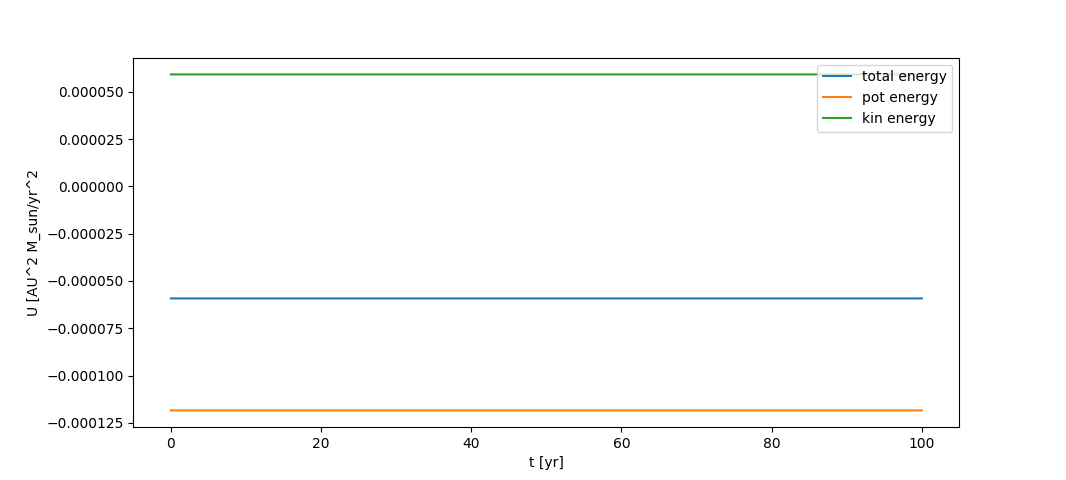
\includegraphics[width=1.0\textwidth]{plots/verlet_energysystem100yr.png}
  \caption{Velocity Verlet method, Time: 100yr, N: 100 000}
\end{figure}
\begin{figure}[H]
  \centering
  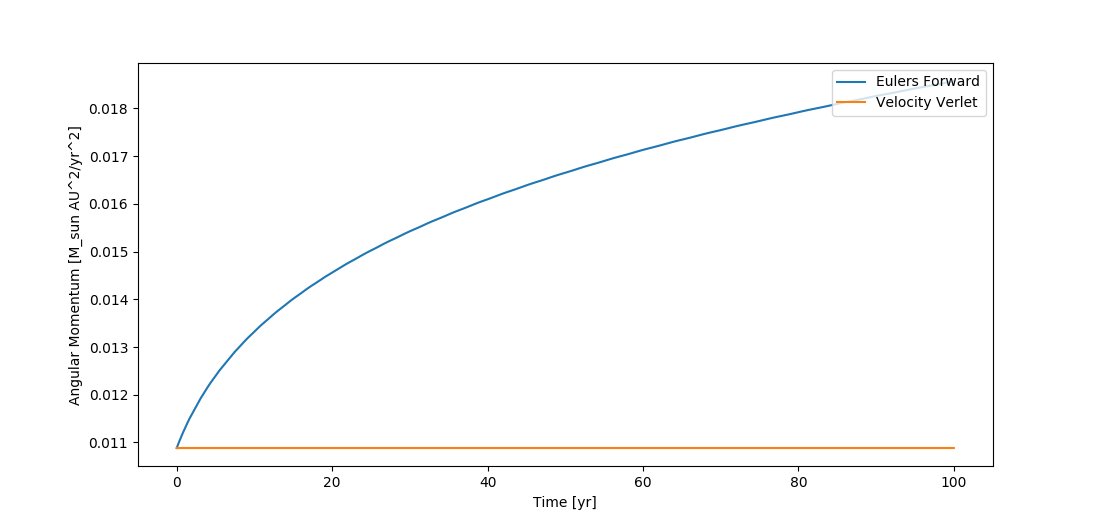
\includegraphics[width=1.0\textwidth]{plots/angular_both.png}
  \caption{Time: 100yr, N: 100 000}
\end{figure}

\section*{Escape velocity}
For a planet starting at $x_0 = 1AU$ the theoretical escape velocity\cite{carroll} can be found from energy conservation:
\begin{align*}
  E_k &= E_p\\
  \frac{1}{2}m_{\Earth}v^2 &= m_{\Earth}\frac{F_G}{m_{\Earth}}r\\
  \frac{1}{2}m_{\Earth}v^2 &= F_G r\\
  m_{\Earth}v^2 &= 2\cdot G\frac{m_{\Sun}m_{\Earth}}{r^2} r\\
  v^2 &= 2G\frac{m_{\Sun}}{r}\\
  v &= \sqrt{2G\frac{m_{\Sun}}{r}}\\
  &= \sqrt{\frac{8\pi^2\left[AU^3/yr^2\right]}{r[AU]}}\\
  &= \sqrt{\frac{8\pi^2}{r}\frac{[AU^2]}{[yr^2]}}\\
  &= 2\sqrt{2}\pi\left[AU/yr\right]\\
\end{align*}
\begin{figure}[H]
  \centering
  \begin{subfigure}{0.5\textwidth}
    \centering
    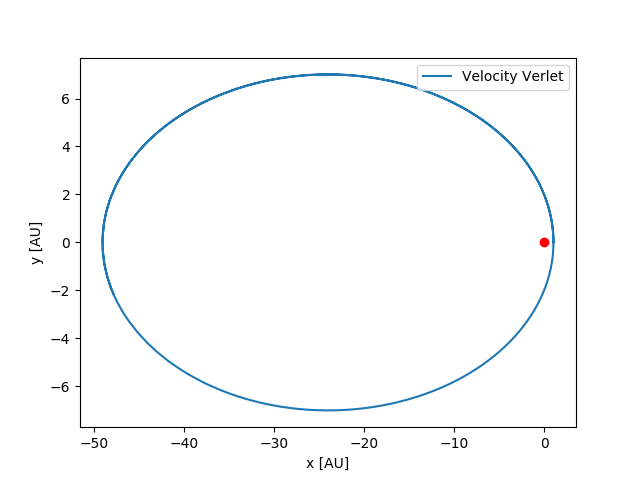
\includegraphics[width=1.0\textwidth]{plots/escape_v2p8pi.png}
    \caption{Velocity Verlet $v_{y_0}=2.8\pi$ (N: 100000, time: 200yr)}
  \end{subfigure}%
  \begin{subfigure}{0.5\textwidth}
    \centering
    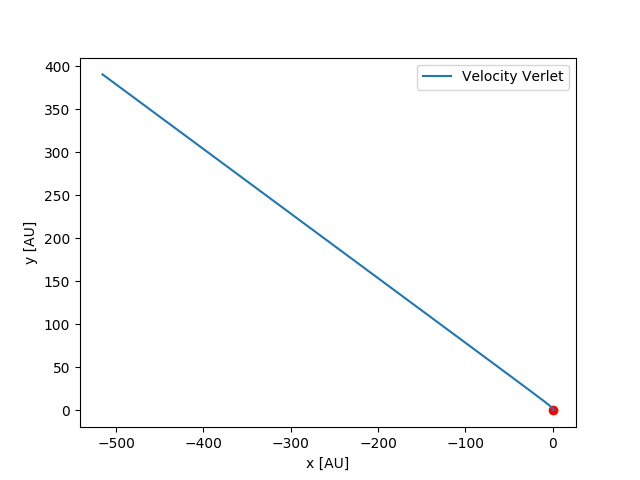
\includegraphics[width=1.0\textwidth]{plots/escape_v3p0pi.png}
    \caption{Velocity Verlet $v_{y_0}=3.0\pi$ (N: 100000, time: 200yr}  
  \end{subfigure}
\end{figure}
{\color[rgb]{1,0,0}The experimental escape velocity $v \approx 8.83 AU/yr$, while the theoretical value was $v\approx 8.89$. This seems reasonable, remembering the total error $O(h^2)$ with $h=0.05$.}

\subsection*{Modifying the gravitational force}
I am now changing the gravitational force to:
\begin{align*}
  F_G &= \frac{GM_{\Sun}m_{\Earth}}{r^{\beta}}\\
\end{align*}
where $\beta \in \left[2,3\right]$.
\begin{figure}[H]
  \centering
  \begin{subfigure}{0.5\textwidth}
    \centering
    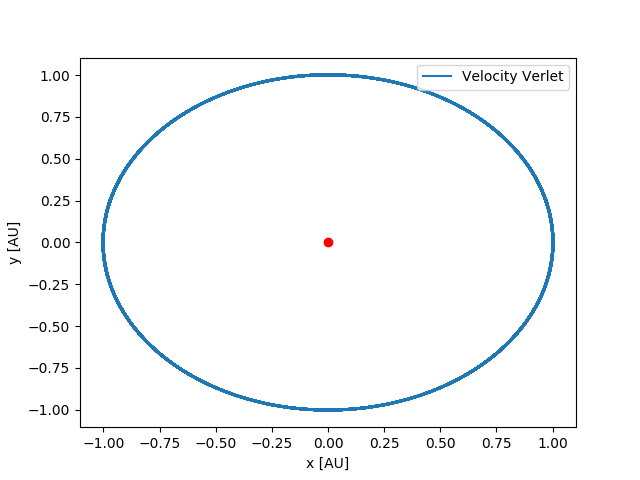
\includegraphics[width=1.0\textwidth]{plots/beta_2p5.png}
    \caption{Velocity Verlet with $\beta =2.5$ \\(N: 10000, time: 100yr)}
  \end{subfigure}%
  \begin{subfigure}{0.5\textwidth}
    \centering
    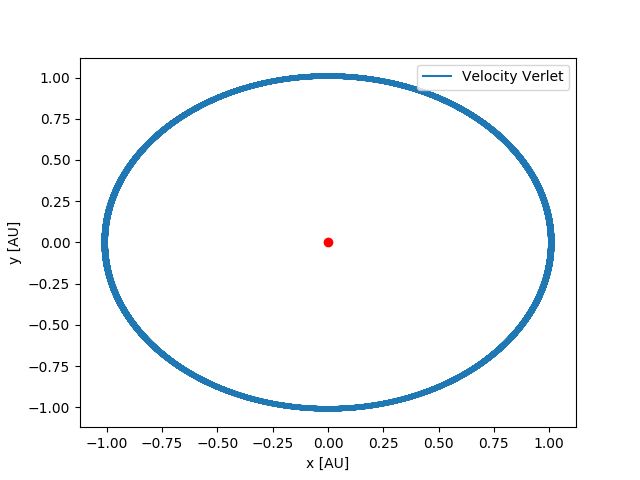
\includegraphics[width=1.0\textwidth]{plots/beta_2p9.png}
    \caption{Velocity Verlet with $\beta =2.9$ \\(N: 10000, time: 100yr}  
  \end{subfigure}
\end{figure}

\begin{figure}[H]
  \centering
  \begin{subfigure}{0.5\textwidth}
    \centering
    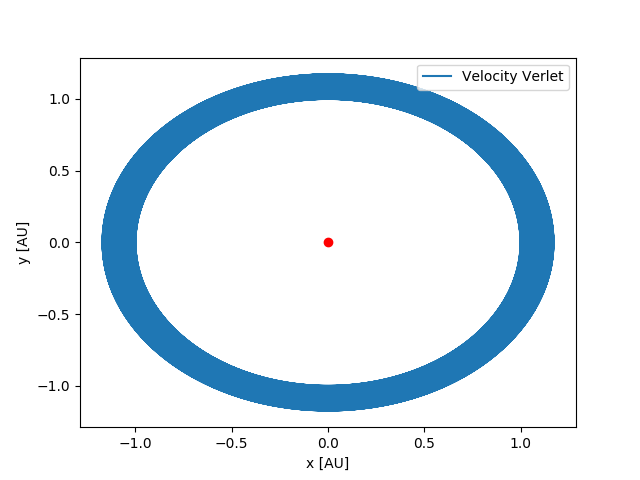
\includegraphics[width=1.0\textwidth]{plots/beta_2p99.png}
    \caption{Velocity Verlet with $\beta =2.99$ \\(N: 10000, time: 100yr)}
  \end{subfigure}%
  \begin{subfigure}{0.5\textwidth}
    \centering
    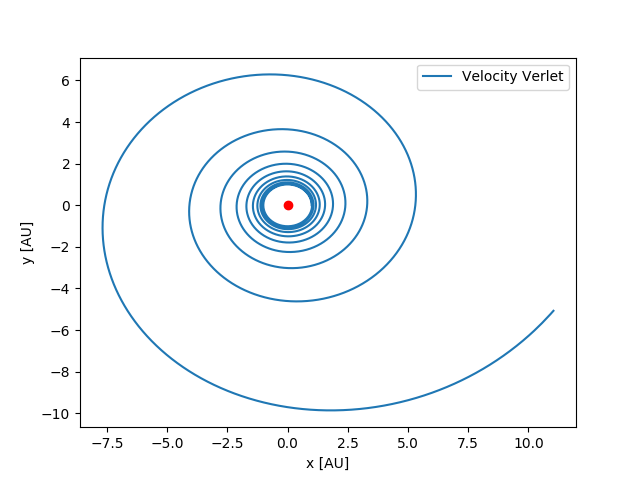
\includegraphics[width=1.0\textwidth]{plots/beta_3.png}
    \caption{Velocity Verlet with $\beta =3.0$ \\(N: 10000, time: 100yr}  
  \end{subfigure}
\end{figure}
\section*{e) The three-body problem}
I am now adding a third object, Jupiter, which I'll give the mass $m_{\Jupiter} = 10^{-3}M_{\Sun}$ and I'll place it at $(x,y)=(5.20AU,0)$. I'll give the planet an initial velocity $v_{y0} =\frac{5.20\cdot2\pi}{11.86}AU/yr$, such that it would be a stable orbit. So far we have seen that the Earth's orbit is stable, but when adding Jupiter we expect an altered motion.
I'll start by showing Jupiters motion around the Sun:
\begin{figure}[H]
  \centering
  \begin{subfigure}{0.5\textwidth}
    \centering
    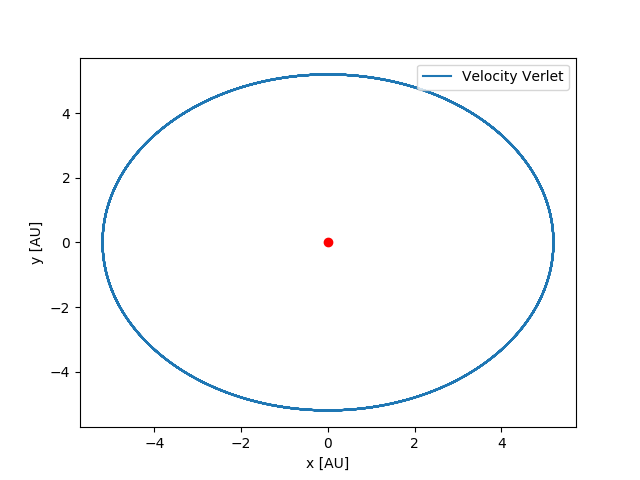
\includegraphics[width=1.0\textwidth]{plots/jupiter.png}
    \caption{Velocity Verlet (N: 100000, time: 100yr)}
  \end{subfigure}%
    \begin{subfigure}{0.5\textwidth}
    \centering
    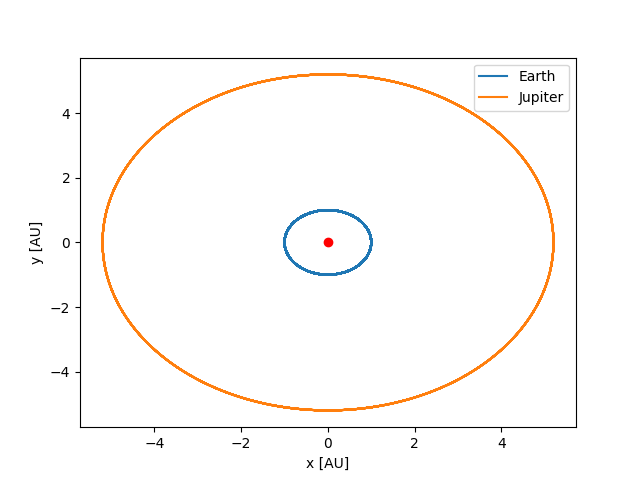
\includegraphics[width=1.0\textwidth]{plots/jupiter_m0p001.png}
    \caption{Velocity Verlet (N: 100000, time: 100yr}  
  \end{subfigure}
\end{figure}
\begin{figure}[H]
  \centering
  \begin{subfigure}{0.5\textwidth}
    \centering
    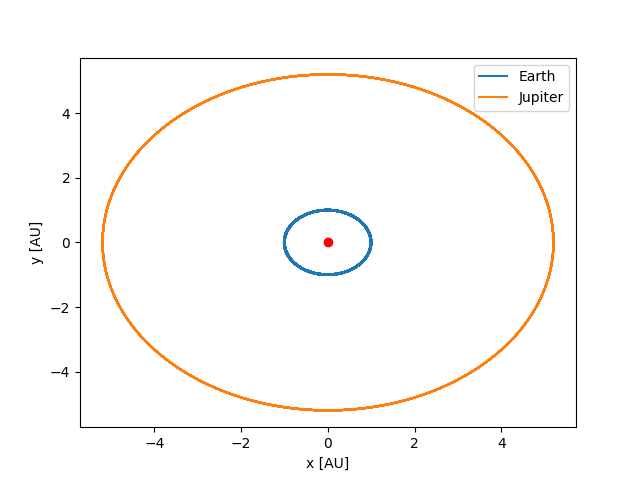
\includegraphics[width=1.0\textwidth]{plots/jupiter_m0p01.png}
    \caption{Velocity Verlet (N: 100000, time: 100yr)}
  \end{subfigure}%
    \begin{subfigure}{0.5\textwidth}
    \centering
    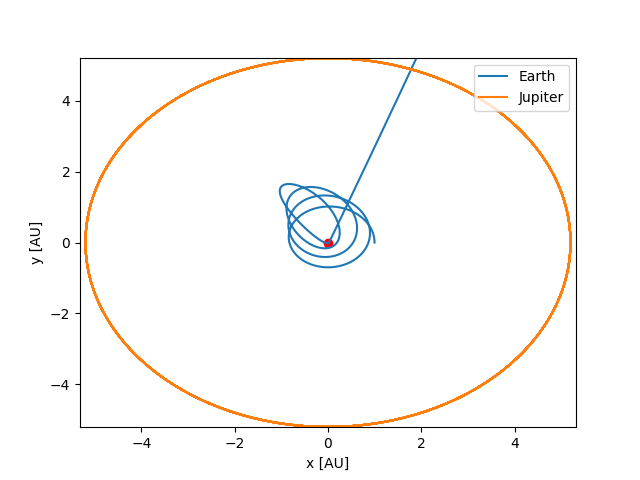
\includegraphics[width=1.0\textwidth]{plots/jupiter_m1p0.png}
    \caption{Velocity Verlet (N: 100000, time: 100yr}  
  \end{subfigure}
\end{figure}
\section*{Final Model}
\begin{figure}[H]
  \centering
  \begin{subfigure}{0.5\textwidth}
    \centering
    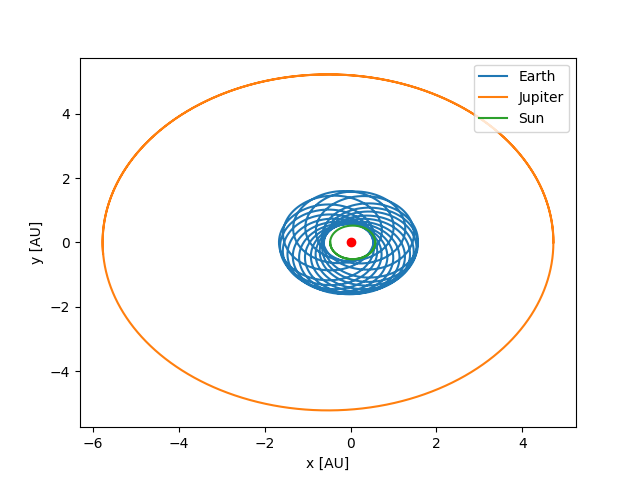
\includegraphics[width=1.0\textwidth]{plots/threebody0p001.png}
    \caption{Velocity Verlet (N: 10000, time: 50yr)}
  \end{subfigure}%
    \begin{subfigure}{0.5\textwidth}
    \centering
    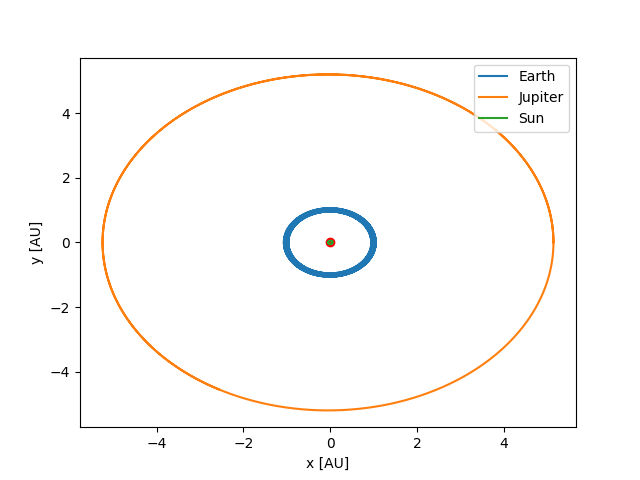
\includegraphics[width=1.0\textwidth]{plots/threebody0p01.png}
    \caption{Velocity Verlet (N: 10000, time: 50yr}  
  \end{subfigure}
\end{figure}
\subsection*{Real data solar system}
\begin{figure}[H]
  \centering
  \begin{subfigure}{0.5\textwidth}
    \centering
    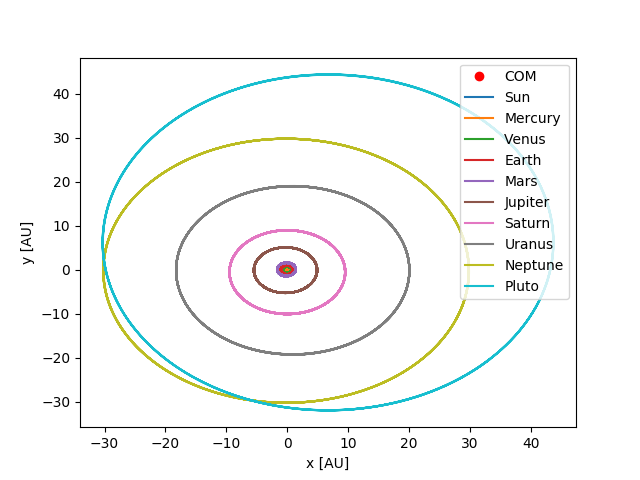
\includegraphics[width=1.0\textwidth]{plots/allplanets.png}
    \caption{Velocity Verlet \\(N: 100000, time: 1000yr)}
  \end{subfigure}%
    \begin{subfigure}{0.5\textwidth}
    \centering
    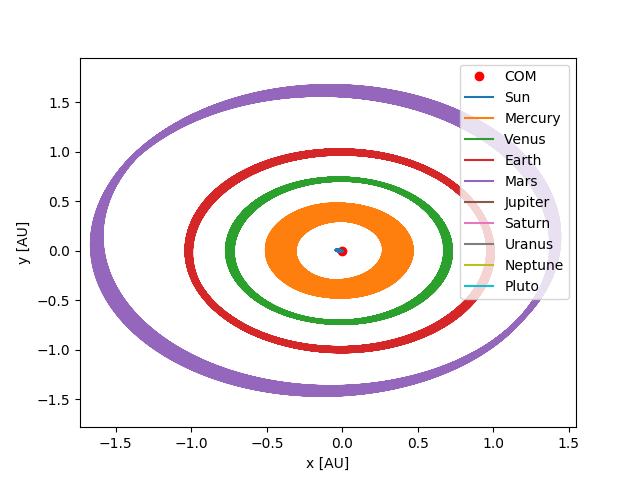
\includegraphics[width=1.0\textwidth]{plots/allplanetszoom.png}
    \caption{Velocity Verlet \\(N: 100000, time: 1000yr}  
  \end{subfigure}
\end{figure}
3D plot
\begin{figure}[H]
  \centering
  \begin{subfigure}{0.5\textwidth}
    \centering
    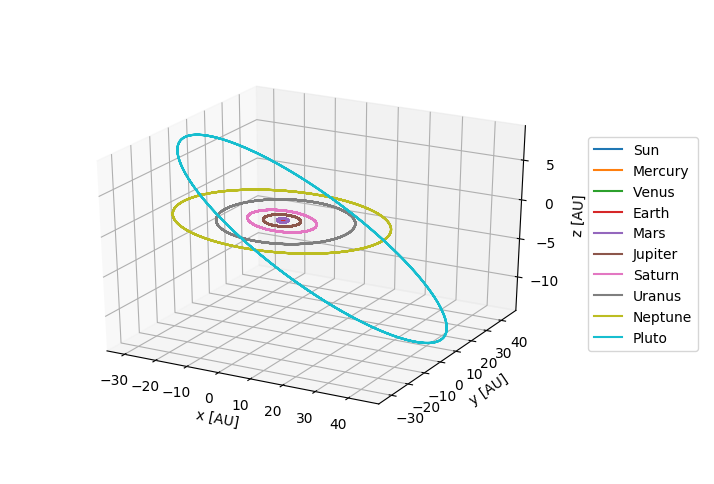
\includegraphics[width=1.0\textwidth]{plots/allplanets3D.png}
    \caption{Velocity Verlet \\(N: 100000, time: 1000yr)}
  \end{subfigure}%
    \begin{subfigure}{0.5\textwidth}
    \centering
    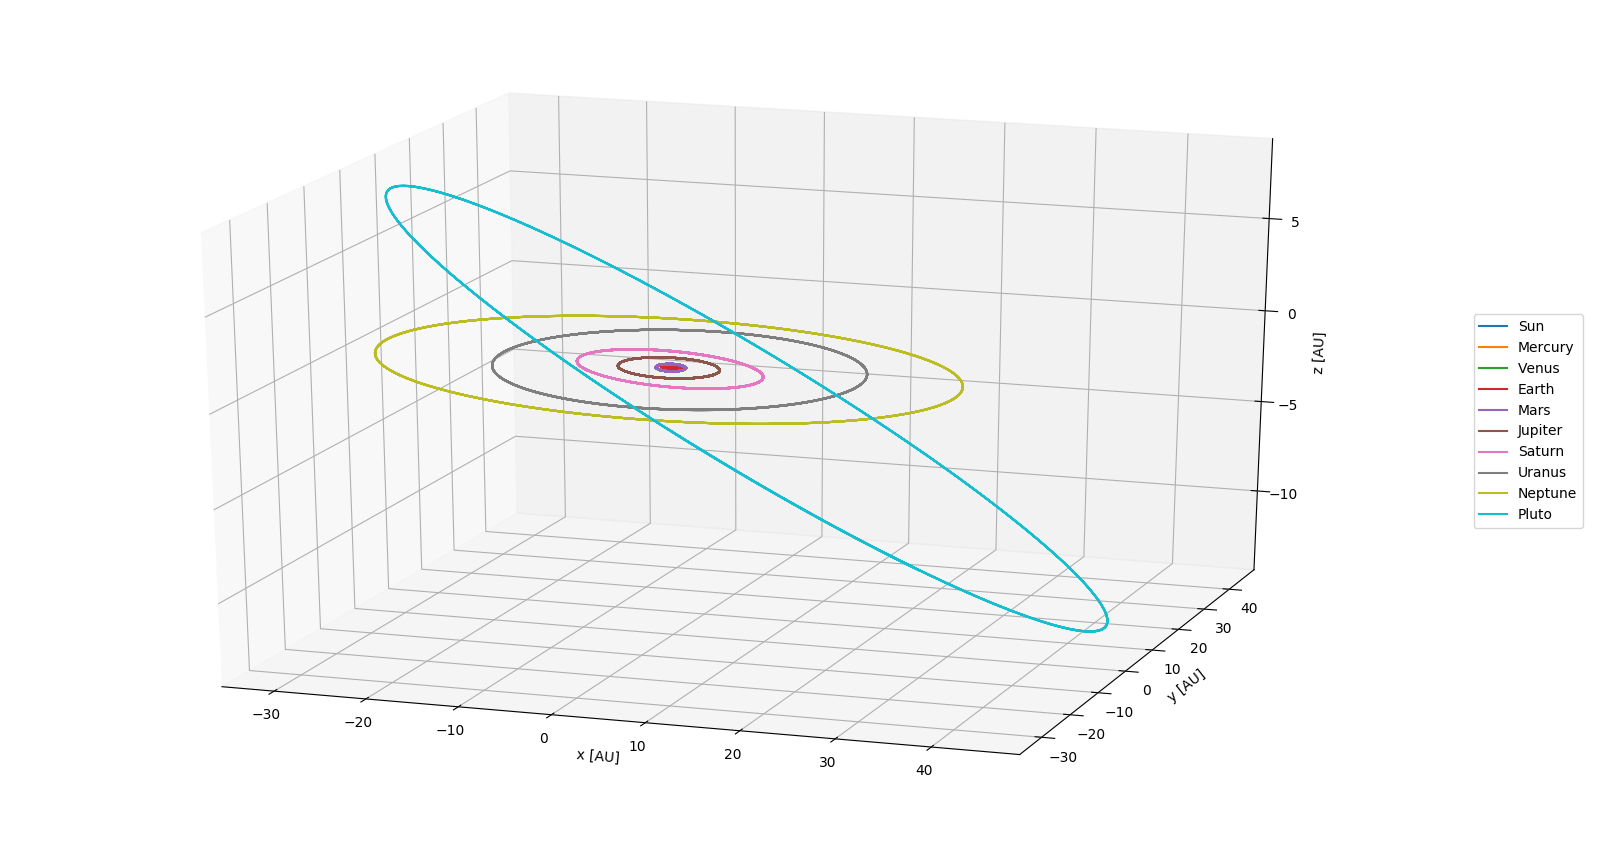
\includegraphics[width=1.0\textwidth]{plots/allplanets3Dbig.png}
    \caption{Velocity Verlet \\(N: 100000, time: 1000yr)}
  \end{subfigure}
\end{figure}
\begin{thebibliography}{9}
\bibitem{carroll}
  Bradley W. Carroll, Dale A. Ostlie
  An Introduction To Modern Astrophysics
  Addison Wesley, San Francisco
  2nd edition,
  2007.
\bibitem{lamport94}
  Leslie Lamport,
  \textit{\LaTeX: a document preparation system},
  Addison Wesley, Massachusetts,
  2nd edition,
  1994.
\end{thebibliography}
\end{document}

